\documentclass[a4paper, 9pt, draft]{amsart}
\usepackage[english]{babel}
\usepackage{amsmath}
\usepackage{amssymb}
\usepackage{amsfonts}
\usepackage{mathtools}
\usepackage{diagbox}
\usepackage{booktabs}
\usepackage{enumitem}
\usepackage{color}
\usepackage{hyperref}
\usepackage{tikz}
\usepackage{accents}
\usepackage{standalone}
\usepackage{bm}
\usepackage{multicol}
\usepackage[font={small,sc}]{caption}

\usetikzlibrary{fit}
\usetikzlibrary{backgrounds}
\usetikzlibrary{positioning}
\usetikzlibrary{decorations}
\usetikzlibrary{decorations.pathmorphing}
\usetikzlibrary{arrows.meta}

\hyphenation{block-chain block-chains}

\hypersetup{colorlinks,
    citecolor=black,
    filecolor=black,
    linkcolor=black,
    urlcolor=blue,
    pdftex}

\setlist[description]{leftmargin=1.2cm, labelindent=\parindent}
\setlist[enumerate]{leftmargin=1.5cm, labelindent=\parindent}

\newcommand*\eg{e.g.\ }
\newcommand*\ie{i.e.\ }

\title[Oscoin]{Oscoin: A Network for Sustainable Open-Source Hosting and Collaboration}
\author{Monadic}
\date{2018}

\newcommand{\oscoin}{\textsc{\small{oscoin}}}
\newcommand{\blake}{\textsc{\small{blake2}}}
\newcommand{\hash}{\mathsc{hash}}
\newcommand{\coin}{$\Theta$}
\newcommand{\mathsc}[1]{\text{\normalfont\scshape#1}}
\newcommand{\tx}[2]{\langle \mathsc{#1}, #2 \rangle}
\newcommand{\tuple}[1]{\langle #1 \rangle}
\newcommand{\cvdots}{\multicolumn{1}{c}{\small{\vdots}}}
\newcommand{\dep}{\xrightharpoondown[e]{d}}
\newcommand{\notice}[1]{{\color{red}#1}}
\newcommand{\todo}{\notice{\texttt{TODO}}}

\newcommand{\rootchain}{\gamma}
\newcommand{\State}{\mathcal{S}}
\newcommand{\Ledger}{\mathcal{L}}
\newcommand{\Orgs}{\mathcal{O}}
\newcommand{\apply}{\Upsilon}
\newcommand{\op}{T}

% Adjust spacing around equations. It can be a bit tight!
\expandafter\def\expandafter\normalsize\expandafter{%
    \normalsize%
    \addtolength{\abovedisplayskip}{2pt}%
    \addtolength{\abovedisplayshortskip}{2pt}%
    \addtolength{\belowdisplayskip}{2pt}%
    \addtolength{\belowdisplayshortskip}{2pt}%
}%

\newenvironment{fig}
  {\par\bigskip\noindent\minipage{\linewidth}}
  {\endminipage\par\bigskip}

% No paragraph indentation after section headers.
\makeatletter
\let\@afterindenttrue\@afterindentfalse
\makeatother

% Issue amend operator.
\DeclareMathOperator{\amend}{\times}

\newenvironment{epigraph}[2][]
{\leftskip=1cm \def\epigraph@author{#2} \smallskip\itshape}
{\par\vspace{0.5em}\normalfont\hfill---\ \epigraph@author\hspace*{0.2cm}\par\medskip}
\makeatother

\setlength{\textwidth}{\paperwidth}
\addtolength{\textwidth}{-4cm}
\setlength{\textheight}{\paperheight}
\addtolength{\textheight}{-5cm}
\calclayout

\begin{document}
\begin{abstract}
    Over the last few decades, with the emergence of open-source software,
    we've experienced an unprecedented acceleration in the development of our
    digital infrastructure, one that has become a new commons -- a public good
    we are now collectively responsible for. But we are all familiar with cases
    like Heartbleed, with developer burn-out, with projects acquired by
    ill-incentivized or incompetent parties. Today, many valuable open-source
    software projects are unable to define themselves in traditional market
    terms, while others find it incompatible with their ethics and struggle
    without financial support. Oscoin is a proposed solution to this problem
    which leverages technology and mechanisms pioneered by early
    crypto-currencies such as Bitcoin and Ethereum.  In a network based
    economy, value should be distributed transparently towards the members who
    contribute value to the network, instead of being captured by a few.  We
    believe that crypto-economies are a means of creating financially
    sustainable decentralized communities.
\end{abstract}
\maketitle

\setlength{\columnsep}{20pt}
\begin{multicols}{2}

\section{Introduction}

\begin{epigraph}{The Open-Source Everything Manifesto}
    \noindent It is in this light that we must recognize that only a restoration of
    open-source culture, and all that enables across the full spectrum of
    open-source possibilities, can allow humanity to harness the distributed
    intelligence of the collective and create the equivalent of heaven on Earth
    -- in other words, a world that works for all.
\end{epigraph}

\noindent \oscoin{} is a protocol and token that attempts to provide a decentralized
hosting solution for open-source code with the means to collaborate on, govern
and fund open-source software projects sustainably, with no central authority
in control.

\subsection{Core Components}

\oscoin{} introduces a few components that, taken together, constitute the core
of the proposed solution.

\begin{description}
    \item[Registry] The registry, formally $\mathcal{R}$, is a
        decentralized service which provides a canonical record of projects and
        organizations known to the network.
    \item[Treasury] The treasury, formally $\mathcal{T}$, is a
        decentralized service with the purpose of funding open-source projects
        of value on the network.
    \item[Network] A decentralized code hosting network, formally
        $\mathcal{N}$, which hosts all the source code known to the network
        in a way that is available and censor-proof.
    \item[Dependency Graph] The dependency graph $\mathcal{D}$, is a global
        graph of all dependencies known to the network, whether these
        dependencies are hosted on the network or hosted externally.
    \item[Oscoin] The \oscoin{} token is a cryptographic token used for value
        exchange in the network.
\end{description}

\subsection{Protocol Overview}

\begin{itemize}
    \item The \oscoin{} network is a decentralized code hosting network
        composed of different kinds of participants, including
        \emph{maintainers}, \emph{contributors} and \emph{operators}.
    \item Maintainers and contributors collaborate around software projects
        organized in code repositories hosted by the network.
    \item Through the registry $\mathcal{R}$, participants discover, support
        and join open-source projects.
    \item Funds available for distribution are first sent to the treasury
        $\mathcal{T}$, before being distributed to chosen organizations.
    \item Token holders are able to pledge a certain amount of tokens towards
        an organization. This has the effect of signaling the treasury that a
        given organization has value to them, influencing the distribution of
        funds.
    \item Organizations are able to use the funds allocated to them for
        whichever purpose they see fit. \emph{Issues} and \emph{smart
        contracts} are used as a means for smart distribution of tokens from
        within an organization, to its constituent members.
    \item Code is attached to issues in the form of \emph{patches}. Issues act
        as the epicenter of change and collaboration around a project.
\end{itemize}
\pagebreak

\section{Background}

To motivate this work, we must first familiarize ourselves with the conditions
in which open-source software is developed, as well as some of the core
technologies and ideas which inspired this work.

\paragraph{The Open-Source Movement.} Software whose source code is publicly
available is called \emph{open-source}. Most of the software we use on a daily
basis relies on free and public code. In an increasingly digitalized society,
these open-source projects have become the foundation of digital infrastructure
underpinning many of our societal goods and services.

Over the last few years, with the emergence of software hosting sites like
GitHub and community sites like Stack Overflow, the open-source paradigm became
the focal point of software development, resulting in the development of
numerous high quality projects wwhich are openly available for anyone to use.
This phenomenon helped companies (a) to reduce lead times and bring products to
the market faster and (b) to recruit talent from a new pool of technologists,
educated on the basis of open-source software.

Today, many open-source projects are started by individuals or small groups of
people solving a personally, socially, or technically relevant problem. By
analysing people's motivations for participating in open-source software
development the following themes emerge: (a) pride in one's work, (b)
reputation, (c) learning, (d) responsibility for something they believe in,
i.e.\ \emph{the project got attention, I have to maintain it}, (e) being part
of a community and (f) financial compensation.

While most open-source software projects start for the reasons above, the ones
that gain momentum require significant resources in time and money to maintain.
This creates a fundamental problem: projects created in the spare time of a
developer are becoming critical public infrastructure. As their projects
gain popularity, developers experience stress and exhaustion trying to keep up
with the requests of the community during their free time, often abandoning
their own projects or burning out under the increased responsibility. Left
unchecked, this leads to a tragedy of the commons~\cite{tragedy-commons} which
is at the core of the problem \oscoin{} attempts to address: financial
sustainability and transparency in the development of open-source software.

% TODO: Talk about the effect on code too!

\paragraph{Version control systems.} At the core of open-source collaboration
is the version control system, or VCS---a system for tracking changes to source
code over time. Version control systems have long been used to manage
open-source software projects and are an essential part of how open-source is
developed, allowing large groups of people to efficiently coordinate around a
project and track contributions individually. In the last two decades, a new
kind of \emph{distributed} VCS has emerged, known as a DVCS, the most popular
of which is \texttt{git}~\cite{git}. But despite the distributed nature
and popularity of \texttt{git}, we are experiencing a new form of
centralization around platforms such as GitHub and GitLab.  What used to be an
open and decentralized process\footnote{Before sites likes GitHub, the majority
of open-source contributions were sent as patches to maintainers on mailing
lists. This is still how the Linux kernel project operates} is now controlled
by a few major players. This is largely due to the convenience of these
platforms, yet few consider the implications of entrusting the world's code to
a commercial organization and relying on a centralized platform which has been
shown to be a single point of failure on more than one occasion.

\paragraph{Blockchain technology.} In 2009, with the publication of the Bitcoin
paper~\cite{bitcoin}, blockchain technology was introduced. Blockchain enables
a peer-to-peer network of participants to agree on the state of a global
\emph{transaction ledger} in the \emph{permissionless} setting. In this
setting, participation in the agreement protocol of the network---also known as
\emph{consensus}---is open and public.

However, what was perhaps the most important discovery took some time to reach
collective consciousness. This was the use of \emph{economic incentives} at the
protocol level. In this model, network operators, or \emph{miners} in the
case of Bitcoin, are incentivized to keep operating the network and to
collaborate with each other, because disagreement has an economic risk.

This inspired a resurgence in protocol thinking and innovation in open network
design, which is the foundation on which we are basing our solution to the
open-source sustainability problem.

Beyond the pressing issues in financial sustainability, open-source projects
organized in a decentralized manner, which is the case for a majority of
blockchain-based projects such as Ethereum and Bitcoin, are lacking the tools
necessary for coordination and decision making around protocol changes.

And although decentralized systems are computationally inefficient, they are
often more resilient, sustainable and available than their centralized
counterparts, properties which are important when designing public
infrastructure.

\pagebreak

\input{sections/network.tex}
\section{Protocol Semantics}
\label{sec:protocol-semantics}

% TODO: Distinguish operations from messages, make sure messages aren't signed.
% TODO: Make sure all operations, ex. around issues are using a message token.

The rules according to which transactions on the \oscoin{} network are
validated comprise a \emph{protocol}. This protocol has a well defined semantics
which we shall describe in this section.

\subsection{Overview} The \oscoin{} protocol is composed of interrelated
\emph{objects} which form a hierarchical graph as seen in Figure
\ref{object-relationships}, and \emph{operations}, which act on these objects.

\medskip

\begin{figure}[htp]
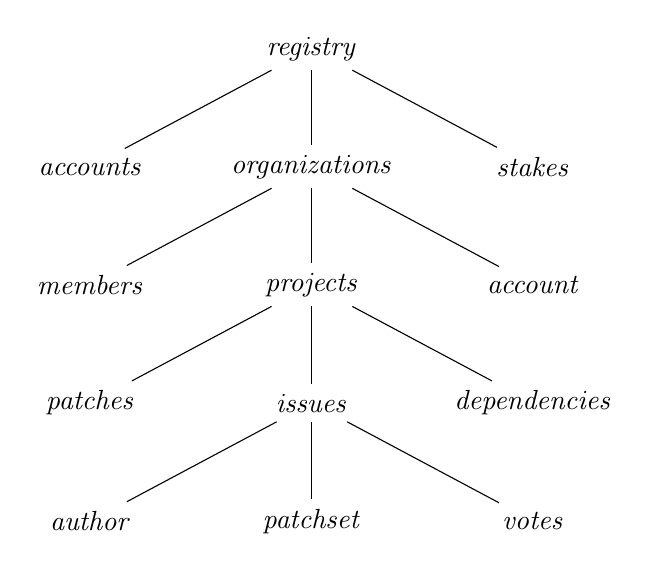
\begin{tikzpicture}[sibling distance=8em]
    \node {\emph{registry}}
        child { node {\emph{accounts}} }
        child { node {\emph{organizations}}
            child { node {\emph{members}} }
            child { node {\emph{projects}}
                child { node {\emph{patches}} }
                child { node {\emph{issues}}
                    child { node {\emph{author}} }
                    child { node {\emph{patchset}} }
                    child { node {\emph{votes}} } }
                child { node {\emph{dependencies}} } }
            child { node {\emph{account}} } }
        child { node {\emph{stakes}} };
\end{tikzpicture}
\bigskip
\caption{Object relationships in the \oscoin{} protocol.
\label{object-relationships}}
\end{figure}

\subsection{Operations and State}
\label{operations-and-state}

% TODO: Call operation messages 'commands'. Then refer to all future
% operations as commands. Move the author, nonce etc. to the command. Make
% operations as a sequence of commands.

Operations are signed messages constructed by participants in the protocol,
which trigger a state transition in the network. A valid operation $T$ takes
the form:
\[
    T \equiv \tuple{T_i, T_m, T_p, T_n}_{\sigma}
\]
where $T_i$ is the identity of the sender of the operation, $T_m$ is the
message, $T_p$ is a reference to a parent operation, such that $T_p
\prec T$, and $T_n \in \mathbb{N}$ taken together with $T_i$ forms a globally
unique operation identifier, such that there can be at most one operation with
a given $\tuple{T_i, T_n}$ tuple. In the remainder of the paper, we shall
use the word \emph{operation} to mean either a tuple $T$, or its message $T_m$.

A valid operation $T$ applied to the current state of
the protocol $\mathcal{S}_e$ at epoch $e$ can be formulated as:
\[
    \mathcal{S}_{e+1} \equiv \delta(\mathcal{S}_e, T)
\]
where $\delta$ is \emph{apply}, the state-transition function.  We can describe
the current state of the network $\mathcal{S}_e$ as a sequence of operations
$\mathcal{L} = T_1 \dots T_e$ applied recursively to an initial empty state
$\varnothing$:
\[
    \mathcal{S}_e \equiv \delta(\dots \delta(\delta(\delta(\varnothing,
    T_1), T_2), T_3), \dots T_e)
\]
The state $\mathcal{S}$ of the protocol is defined as:
\[
    \mathcal{S} \equiv \tuple{\mathcal{A}, \mathcal{O}, \mathcal{D}, \mathcal{L}} \\
\]
where $\mathcal{A}$ is the set of accounts (\ref{accounts}), $\mathcal{O}$ is
the set of organizations known to the protocol (\ref{orgs}), $\mathcal{D}$ is
the set of dependencies between projects (\ref{dependencies}) and $\mathcal{L}$
is the sequence of operations which have been applied to $\mathcal{S}$. It is
thus possible to reconstruct $\mathcal{S}$ from $\mathcal{L}$ via the $\delta$
function, as seen above.

\subsection{Patches}
\label{patches}

The fundamental product or \emph{artifact} of the \oscoin{} network is code, or
source code. Our protocol defines the \emph{patch} primitive as the atomic unit
of code. A patch is a set of metadata and code changes, or \emph{changeset},
that can be applied to an existing body of code, or \emph{context}, to modify
it. We define a patch $P$ as the tuple $\tuple{ P_a, P_m, P_f}$, where $P_a$ is
the author of the patch, $P_m$ is the patch metadata and $P_f$ is the
changeset. A set of patches in no particular order is called a \emph{patchset}.

Patches can be composed sequentially, taking an initial context $A$ into
a modified context $B$. The empty context is defined as $\varnothing$, such
that there exists a mapping $P_f \varnothing \mapsto P_f$. Let $f \prec g
\prec h$ be an ordered sequence of patches, then the formulation:
\[
h \cdot g \cdot f : A \to B
\]
is the in-order composition of patches $f$, $g$ and $h$, taking an initial
context from $A$ to $B$.

% TODO: Contexts form a free monoid?
% TODO: Reference patch theory.

\subsection{Issues}
\label{issues}

On the \oscoin{} network, collaboration on code takes place through \emph{issues};
and since project governance is specified in code---through the use of
\emph{smart contracts}---organizational decisions are also made through issues.

% TODO: Remove reference to smart contracts!

An issue $I$ is described at epoch $e$ by the tuple:
\[
    \big<\tuple{I_a, I_t, I_b, I_o, I_r, I_P}_{\sigma}, I_s, I_V \big>_e
\]
where $I_a$ is the issue author, $I_t$ is the title or subject of the issue,
$I_b$ is the description in plain text of the issue, $I_o$ is a list of
operations to be applied when $I_s$ changes, $I_r$ is the issue resolution
function, $I_P$ is the patchset attached to the issue, $\sigma$ is the
signature of $I_a$, $I_s \in \{open, closed, accepted, rejected\}$ is the
current state of the issue and $I_V$ is the set of votes on the issue. The
initial value of $I_s$, $I_{s_0} = open$, the initial value of $I_V$, $I_{V_0}
= \varnothing$ and the initial value of $I_P$, $I_{P_0} = \varnothing$.  A list
of valid state transitions between any two states $I_s$ and $I_{s'}$ can be
found in Table \ref{issues-valid-transitions}.

\begin{table}[hbt]
    \caption{Valid state transitions.\label{issues-valid-transitions}}
    \begin{tabular}{rcl}
        \toprule
        $I_s$      & $\to$ & $I_{s'}$ \\
        \midrule
        $open$     & $\to$ & $accepted$ \\
        $open$     & $\to$ & $rejected$ \\
        $open$     & $\to$ & $closed$ \\
        $closed$   & $\to$ & $open$ \\
        \bottomrule
    \end{tabular}
\end{table}

The patchset $I_P$ attached to an issue represents a set of proposed changes to
some project, while the subject $I_t$ and body $I_b$ of the issue provide a
description of the changes contained in $I_P$. Issue \emph{resolution} is the
process of voting on an issue with the aim to move to an \emph{accepted} or
\emph{rejected} state.

Issues can be voted on with the \textsc{voice} operation. When an issue receives
a new vote, it is added to $I_V$. A vote $v$ is represented by the tuple
$\tuple{v_i, v_a, v_{\omega}, v_e}_{\sigma}$ where $v_a$ is the voter,
$v_i$ is the issue being voted on, $v_{\omega} \in \{accept, reject\}$ and
$v_e$ is the epoch $e$ at which the vote is valid.

When a certain threshold of votes is reached, an issue transitions to either an
\emph{accepted} or \emph{rejected} state. Given an open issue $i$, the rules of
issue resolution are defined by the function $i_r : I \to I$, applied to the
issue $i$ for every vote added to $i_V$.

\subsubsection{Amendments}

An issue $I$ where $I_s = open$ can be amended with the \textsc{amend}
operation, or $\amend$. Only $I_t$, $I_b$, $I_o$, $I_r$ and $I_P$ can be
amended.  Amending an issue creates a new empty set of votes $V'$, ensuring two
versions of a given issue never share a set of votes. Formally, amendment is
defined as:
\begin{align*}
    I \amend{} \langle I_a, t', b', o', r', P' \rangle_{\sigma} \equiv
    \big<\langle I_a, t', b', o', r', P' \rangle_{\sigma}, I_s, \varnothing
    \big>, \qquad I_s = open
\end{align*}

% TODO: The amendment should include the issue it is amending.

\subsubsection{Accepted Issues} When an issue has been accepted by a majority
of votes, the issue transitions permanently into an \emph{accepted} state. The
steps taken by the protocol are as follows:

\begin{enumerate}
    \item The issue's state $I_s$ is set to \emph{accepted}.
    \item The issue is \emph{frozen}, such that no further amendments or state
        changes are possible.
    \item The list of operations $I_o$ belonging to the issue are executed by
        the protocol.
    \item The issue's \emph{patchset} $I_P$ is permanently added to the code
        project it pertains to. Note that a patchset may contain individual
        patches pertaining to different projects, in which case the patches are
        applied individually to their respective projects.
\end{enumerate}

\subsubsection{Rejected issues} When an issue is rejected,
\begin{enumerate}
    \item The issue transitions to a \emph{rejected} state.
    \item The issue is frozen so that no further amendments or state
        transitions are possible.
    \item The list of operations $I_o$ belonging to the issue are executed by
        the protocol.
\end{enumerate}

\subsubsection{Closed issues} When an issue is closed, its state changes to
\emph{closed} until it is re-opened. No operations from $I_o$ are run, since
an issue can be opened and closed many times. Only the author $I_a$ of an issue
can close it.

\subsection{Value}

To enable the transfer of value in the network, the protocol defines a scarce
currency we shall refer to in the remainder of this paper as~\coin{}, or
\oscoin{}.

\subsubsection{Supply}

The supply of \coin{} is subject to an inflation $e_{\iota} \in \mathbb{N}$,
carried out by the protocol every epoch $e$, and determined by a function $f :
e \to e_{\iota}$, such that
\[
    \lim_{e\to\infty} f(e) = 0
\]

\subsubsection{Accounts}
\label{accounts}

Currency is held in \emph{accounts} which can be unlocked by the signature of
the account holder. Accounts have addresses which are used to send and receive
\coin{}. The set of all accounts is known as $\mathcal{A}$.

\subsubsection{Transfer}

Value can be transfered from one account to another with the \textsc{send}
message, formally defined as $\tx{send}{a_{s}, a_{r}, n}$, where $a_{s}$ and
$a_{r}$ are the \emph{sender} and \emph{recipient} address between which the
value should be transfered and $n$ is the value to transfer.  To be valid, a
\textsc{send} operation must be signed by the owner of $a_{s}$.

\subsubsection{Bonding}

Value can be locked in the system via an operation called \emph{bonding}.
This operation turns \emph{liquid} value into \emph{bonded} value, preventing
them from being moved for a certain amount of time, and can be used to perform
security deposits or other forms of commitment which require a collateral or
pledge. Bonding and unbonding operations are performed with the
\textsc{bond} and \textsc{unbond} messages defined as:
\[
    \tx{bond}{a, a_b, n} \qquad \tx{unbond}{a, a_b, n}
    \medskip
\]
where $a$ is the address from which to withdraw the value for bonding, $a_b$ is
the address where the value is to be bonded and $n$ is the value to bond. When
the \textsc{unbond} operation is used, an unbonding period $e_u$ is started,
measured in epochs. Once $e_{u}$ epochs have passed, the value is withdrawn
from the bonding address $a_b$ and credited back to $a$.

\subsection{Organizations}
\label{orgs}

An organization $O$ is described by the tuple:
\[
    \tuple{O_{id}, O_{a}, O_R, O_M}
\]
where $O_{id}$ is the organization's identifier, $O_a$ is its account, $O_R$ is
the set of repositories under $O$ and $O_M$ is the set of members belonging to
the organization. We can relate patches (\ref{patches}) and issues
(\ref{issues}) to repositories with the equations:
\begin{align*}
    O_R & \equiv \{R_1, R_2, \dots, R_n\}         \\
    R   & \equiv \tuple{R_{id}, R_I, R_P}         \\
    R_I & \equiv \{I_1, I_2, \dots, I_n\}         \\
    R_P & \equiv \tuple{P_1, P_2, \dots, P_n}
\end{align*}
where $R_{id}$ is the repository's identifier, $R_I$ is the set of issues
related to $R$, and $R_P$ is the sequence of patches composing its codebase.

The set $\mathcal{O} = \{O_1, O_2, \dots, O_n\}$ is the set of all organizations
known to the protocol.  Let $o$ be an organization, then $\tx{register}{o}$ is
an operation that registers $o$ and makes it known to the protocol such that:
\[
    \delta_o(\mathcal{O}, \tx{register}{o})
    \equiv \mathcal{O} \cup \{o\}
\]
where $\delta_o$ is a sub-function of $\delta$, and defines state-transitions
in $\mathcal{O}$.

\subsection{Dependencies}
\label{dependencies}

A project $a$ depends on a project $b$ at epoch $e$ if it references $b$
or parts of $b$. Formally, we represent this as:
\[
    D \equiv \tuple{D_a, D_b, D_e} \qquad or \qquad a \dep b
\]

% TODO: dependencies with \overrightarrow{AB}, like vectors.

Let $\accentset{*}{R}$ be the set $O_{1_R} \cup O_{2_R} \cup \cdots \cup
O_{n_R}$ of all projects accross all organizations, and $\mathcal{D}_e$ be the
set of all dependencies at epoch $e$, then:
\[
    \mathcal{D}_e \equiv \{(a, b) : a \in \accentset{*}{R}
    \land b \in \accentset{*}{R}
    \land a \dep b \}
\]

Dependencies are recorded with the $\tx{depend}{D_a, D_b, D_e, D_{e'}}$
operation, which records a dependency between $a$ and $b$ for each epoch $x$
where $e \leqslant x \leqslant e'$.

\section{The Dependency Graph}
\subsection{The Dependency Game}

% TODO: "As an individual entity, you are not a party to the flow of value
% in the economy."

To incentivize the building of a dependency graph for open-source, we create a
mechanism which rewards participants for identifying dependencies correctly and
punishes them for acting maliciously.

There are two types of players in the game: \emph{proposers} and
\emph{verifiers}.  The former propose a dependency between two projects which
they believe to be valid, and place a security deposit $G_{\delta}$ which they
are prepared to lose if they are lying. The later verify proposals by casting a
vote which can have either of two values: $1$ (\emph{true}), for proposals
believed to be valid, and $0$ (\emph{false}), for proposals considered
invalid. Verifiers who manage to agree on $G_d$ without communicating
are each rewarded with an amount of tokens $\delta$.

% TODO: Problem: how to stop validators from communicating.
% TODO: Automation for proposers and validators.
% We recall that a dependency is represented by the tuple $\tuple{D_a, D_b, D_e}$
% described in~\S~\ref{dependencies}.

A dependency game $G$ is initiated by a proposer $G_p$ and progresses in a
sequence of rounds $G_r \equiv r_1 \dots r_n$, where $n \geqslant 1$. Each
round $r$ attempts to resolve the dependency $G_d$ (the ``proposal''), by
either marking it \emph{true} or \emph{false}, and involves two verifiers,
their votes $r_{v_1}$ and $r_{v_2}$, and their deposits $r_{\delta_1}$ and
$r_{\delta_2}$. When $r_{v_1} \equiv r_{v_2}$, the game ends.  Formally, we
have:
\begin{align*}
    G      & \equiv \tuple{G_d, G_p, G_{\delta}, G_r} \\
    G_r    & \equiv \{r_1, \dots, r_n\} \\
    r      & \equiv \tuple{r_{v_1}, r_{v_2}, r_{\delta_1}, r_{\delta_2}} \\
    r_v    & \in \{0, 1\} \\
\end{align*}
The game starts with an initial state $G_0$, where $G_{0_r} = \varnothing$.
The first round $r_1$ is played as such, where $r \equiv r_1$:

\begin{enumerate}
    \item Two players $r_{p_1}$ and $r_{p_2}$ with deposits $r_{\delta_1}$ and
        $r_{\delta_2}$ are selected at random to become verifiers, and
        presented with $G_d$. Their identities are not revealed to one another.
    \item $r_{p_1}$ and $r_{p_2}$ each cast a vote $r_{v_1}$ and $r_{v_2}$
        signaling whether they believe $G_d$ to be \emph{true} or \emph{false}.
        The votes are not revealed until both players have cast their vote.
\end{enumerate}

Now, the system is in either of three states:

\begin{enumerate}
    \item[(a)] $r_{v_1} \equiv r_{v_2}$, \qquad $r_{v_1} = 1 \; \wedge \; r_{v_2} = 1$
    \item[(b)] $r_{v_1} \equiv r_{v_2}$, \qquad $r_{v_1} = 0 \; \wedge \; r_{v_2} = 0$
    \item[(c)] $r_{v_1} \not\equiv r_{v_2}$
\end{enumerate}

If we find ourselves in state (a), all deposits are returned to the
participants, and $r_{p_1}$, $r_{p_2}$ and $G_p$ are rewarded.  In the case of
(b), the proposer loses their deposit $G_{\delta}$, and it is split between
$r_{p_1}$ and $r_{p_2}$.  Finally, in (c), the verifiers have voted
differently, and there is no way to resolve the round.  Therefore we proceed
with the following:

\begin{enumerate}
    \item A new round is initiated with the same proposal $G_d$, and two new
        verifiers $r_{p_3}$ and $r_{p_4}$, which are picked at random:
        \begin{equation*}
            r_2 \equiv \tuple{r_{v_3}, r_{v_4}, r_{\delta_3}, r_{\delta_4}}
        \end{equation*}
    \item Again, we have three outcomes:
        \smallskip
        \begin{enumerate}
            \item[(a)] $r_{v_3} \equiv r_{v_4}$, \qquad $r_{v_3} = 1 \; \wedge \; r_{v_4} = 1$
            \item[(b)] $r_{v_3} \equiv r_{v_4}$, \qquad $r_{v_3} = 0 \; \wedge \; r_{v_4} = 0$
            \item[(c)] $r_{v_3} \not\equiv r_{v_4}$
        \end{enumerate}
        \smallskip
        In both outcomes (a) and (b), $r_{v_3}$ and $r_{v_4}$ settle the
        previous round $r_1$, by forming a $\frac{3}{1}$ majority vote for
        either $1$ or $0$. This causes the minority voters to lose their
        deposits to the majority. Note that in each round where agreement is
        not reached, we have an additional $2\delta$ at stake.

        In the case of (c), we proceed the same way as in $r_1$, initiating a
        new round with new verifiers.  Each additional round increases the
        total value at stake. Since additional rounds do not cost the system
        more, there is no limit to the number of rounds.
\end{enumerate}

\begin{table}[hbt]
    \caption{Outcomes for $G$ when $G_d$ was voted \emph{valid}}
    \begin{tabular}{lccrrrc}
    \toprule
                  & \multicolumn{2}{c}{Vote} & \multicolumn{3}{c}{Reward} & Cost                    \\
    \midrule
                  & $r_{v_i}$  & $r_{v_j}$   & $r_{p_i}$ & $r_{p_j}$ & $G_p$    &                   \\
    \addlinespace[0.5em]
        $r_{n-2}$ & $1$        & $0$         & $\delta$  & $-\delta$ &          & $0$               \\
        $r_{n-1}$ & $0$        & $1$         & $-\delta$ & $\delta$  &          & $0$               \\
        $r_{n}$   & $1$        & $1$         & $\delta$  & $\delta$  & $\delta$ & $3\delta$         \\
    \bottomrule
    \end{tabular}
\end{table}

\begin{table}[hbt]
    \caption{Outcomes for $G$ when $G_d$ was voted \emph{invalid}}
    \begin{tabular}{lccrrrc}
    \toprule
                  & \multicolumn{2}{c}{Vote} & \multicolumn{3}{c}{Reward} & Cost                     \\
    \midrule
                  & $r_{v_i}$  & $r_{v_j}$   & $r_{p_i}$ & $r_{p_j}$ & $G_p$     &                   \\
    \addlinespace[0.5em]
        $r_{n-2}$ & $1$        & $0$         & $-\delta$ & $\delta$  &           & $0$               \\
        $r_{n-1}$ & $0$        & $1$         & $\delta$  & $-\delta$ &           & $0$               \\
        $r_{n}$   & $0$        & $0$         & $\delta$  & $\delta$  & $-\delta$ & $\delta$          \\
    \bottomrule
    \end{tabular}
\end{table}


\input{sections/issues.tex}
\input{sections/economy.tex}
\section{New Mechanisms for Funding Open-Source}

\subsection{Overview}

Funding is done in the form of cryptographic tokens. These tokens are tradeable
within and without the network.

We can distinguish between two forms of funding: continuous and ad hoc. The
former is carried out automatically by the system, while the latter is carried
out by individuals on the network.

Continuous funding is specified via smart-contracts external to the protocol.
These contracts will be up for discussion with the community and subject to
change as the network evolves.

Ad hoc funding includes donations, bounties and one-time rewards for good work.
These rewards are defined by project owners via smart-contracts, essentially
allowing them to incentivize any interaction around their code (bug reports,
code review, closing issues, etc.)

In the continuous model, projects receive funds and are in charge of
redistributing them to their contributors. The second part can take place
automatically, via project-specific smart-contracts, or on an ad hoc basis, via
per-project funds used by project owners to pay individual contributors.

\subsubsection{Continuous funding}

In this model, tokens are created on every block as part of the \emph{coinbase
transaction.} These newly-minted tokens supply a network-wide treasury which is
used to fund projects. As with Bitcoin, the assumption is that the dilution
creates more value than it takes away from existing token holders. Through this
model, we create a continuous supply of tokens.

Community-vetted means that projects apply for a certain amount of funding per
epoch, and go through a vetting process for approval. Once approved, funds are
dispensed from the treasury to the project’s smart-contract address every
epoch. This approach is reliable, but difficult to scale. Thankfully, it is
easy to incentivize users to perform the vetting process by distributing a
share of the minted tokens to those who do the work.

Community-vetted funding works similarly to existing open-source funds, with an
application process and jury. The difference being the provenance of the funds.

\subsubsection{Tokenization}

Besides the obvious ability to set bounties on issues and donate to
projects—features which are available in current systems—we give projects the
option to tokenize.

Tokenizing a project means exchanging \oscoin{} for project tokens at a fixed
price. Only the project owner can mint new project tokens. We call these
shares.

Project shares are only tradeable within the \oscoin{} network, and can be
compared to ERC20 tokens on the Ethereum network.

Once a project has its own shares, it can use them to incentivize
contributions. It also becomes possible for users to ‘invest’ in a project by
buying shares from the owner.

These shares, depending on the project, can have utility attached to them, such
as voting power. This is up to the project to determine, but users who are very
invested in certain projects might want to have a ‘say’ in project direction.

Another way to think about shares is as an alternative to donation systems. A
user is always (subject to liquidity) able to sell their shares and re-invest
the money in a different project. This isn’t possible with donations.

To conclude, project tokenization allows one-time fundraisers to be carried out
with minimal setup.

\subsubsection{Bounties and Ad-hoc funding}

\subsubsection{Integration with other crypto-tokens}

In certain cases such as Dash or Cardano, cryptocurrencies already have a
treasury system from which they can pay contributions.

These projects usually build their own platform for funding proposals and
paying contributors.

As an alternative, projects such as these could use the \oscoin{} platform to
manage proposals and contributors, and focus on building their core protocol.
For this to work, we can imagine treasury funds being sent regularly to an
exchange to be converted to \oscoin{}. The \oscoin{} would then be deposited in the
project’s wallet on the \oscoin{} blockchain, and used to pay contributors there.

% TODO: Talk about pegging. Saying one oscoin-ADA can always be exchange for an ADA.

\subsection{The Open-Source Registry}

% A \emph{registry} is part of the state $\mathcal{S}$ kept by the protocol, and
% provides a canonical list of entities known to the protocol under a certain
% prefix. Adding an entry to a registry is accomplished with the
% \textsc{register} operation, defined as:
% \[
%     \langle \textsc{register}, r, m, d \rangle
% \]
% where $r$ is the registry under which this entry should be added, $m$ is the
% name being registered and $d$ is the digest of an object $m$ should point to.

\subsubsection{Registration}
A user wishing to deploy a new organization on \oscoin{} starts by sending a
$\langle \mathbf{register}, name \rangle$ transaction to the root chain. The
transaction is processed and an org with the given name is temporarily added
to the registry, with a new \oscoin{} address $\mathcal{A}$.

For the org to remain in the registry, it has to be backed by a minimum amount
of \oscoin{}. Any user can back an org by sending \oscoin{} to $\mathcal{A}$.
Doing so locks the tokens for a minimum amount of time. Tokens deposited and
locked in this manner are called \emph{bonded tokens}. When enough tokens are
bonded in $\mathcal{A}$ to clear the minimum, the org is considered registered.

Note that there is no `unregister' transaction for organizations, since
withdrawing all existing deposits under the name and waiting a certain amount
of blocks accomplishes this.

\subsubsection{Validation}
For an org to have its transactions validated and its blocks minted, it needs
to acquire validators. The process of registration discussed above is all that
is required to incentivize validators to validate an org chain.

\subsubsection{Block reward and bonded tokens}

Since bonded tokens are illiquid, and the circulating supply of tokens is
inflated every block through minting, bonded tokens slowly lose their value
over time as they get dilluted and can't be spent. To componensate for this,
part of the block reward is payed back in interest, proportional to the bonded
stake.

\subsubsection{Staking}

The function of bonding however is not only to get organizations registered.
Bonded tokens generate interest for the orgs and dividends for the token holders.

Let $\phi$ be the inflation per block allocated for interest payments and $s_i$
be the amount of stake bonded in $Acme$ by user $i$. The total amount bonded in
$Acme$ is thus $s_1 + s_2 + \cdots + s_n$ where $n$ is the number of user
deposits.  Let $S$ be the total amount of bonded stake across \emph{all} orgs.
The share of tokens bonded by $i$ as a proportion of the total is thus
$\frac{s_i}{S}$. To calculate the amount of interest tokens $Acme$ would
receive from $i$, we simply multiply the share of bonded tokens with $\phi$, or
$\phi \frac{s_i}{S}$. Furthermore, the total amount of interest $Acme$ would
receive is

\begin{equation*}
\sum_{i=1}^n s_i \cdot \frac{\phi}{S}
\end{equation*}

{\color{red}
    The stake behind an org is the total stake validators have to match. So if
    10 tokens are staked, we can split it as 3-3-2-2. Now a validator can stake
    either 3 or 2 behind this org. Once four validators have staked, the slots
    are filled. However, more validators can keep on staking and function as
    replacements. Validators are selected at random so that a single validator
    has no incentive to fill all slots.

    How to make sure that an org is validated by multiple physical validators
    and not a single validator with 4 keys? Perhaps there is a fixed cost to
    staking of 1, so if you stake 10, you get 9 in reward. But if you stake
    2-2-2-2-2, you get only 5 in reward. So you're incentivized to bigger and
    fewer stakes. Is this good for the network? Perhaps it's adjustable. This
    works if there's too much to stake and not enough places to stake. If there
    isn't enough to stake, then many orgs will go without stake as validators
    focus on large stakes only. A way out is to have a max stake for orgs. Ex.
    you can't create slots > 10, so you're force to split things up a little.
}


\section{Network Protocol and Architecture}

The \oscoin{} network protocol is a realization of the protocol semantics
described in \S~\ref{sec:protocol-semantics}, into the asynchronous network
model.

\subsection{Overview}

The \oscoin{} network is composed of a set of nodes, or \emph{replicas}, which
execute a protocol $\mathcal{P}$. Together, these nodes form a \emph{Replicated
State Machine} with a set of states $\State^*$, a transition function $\apply$,
a starting state $\State_0$, a set of inputs $B_0 \dotso B_n$, and an empty set
of outputs.

% TODO: Are we using the 'P' variable?

Participation in the network protocol is \emph{open} (\ie ``permissionless''),
which makes the replica set dynamic. To achieve consensus in the permissionless
setting, we make use of \emph{blockchains}~\cite{bitcoin} as the underlying
replicated data-structure, with the assumption that a greater than $50\%$
majority of replicas are honest.  However, unlike other blockchain protocols,
we describe a ``block-lattice'' design (Figure~\ref{block-lattice}.) in the
spirit of \cite{raiblocks}, with causal consistency guarantees
\cite{causal-consistency} and partial ordering across chains.

\subsubsection{Block-lattice Architecture}

\begin{figure}[hbp]
    \documentclass[tikz]{standalone}

\usetikzlibrary{fit}
\usetikzlibrary{positioning}

\begin{document}
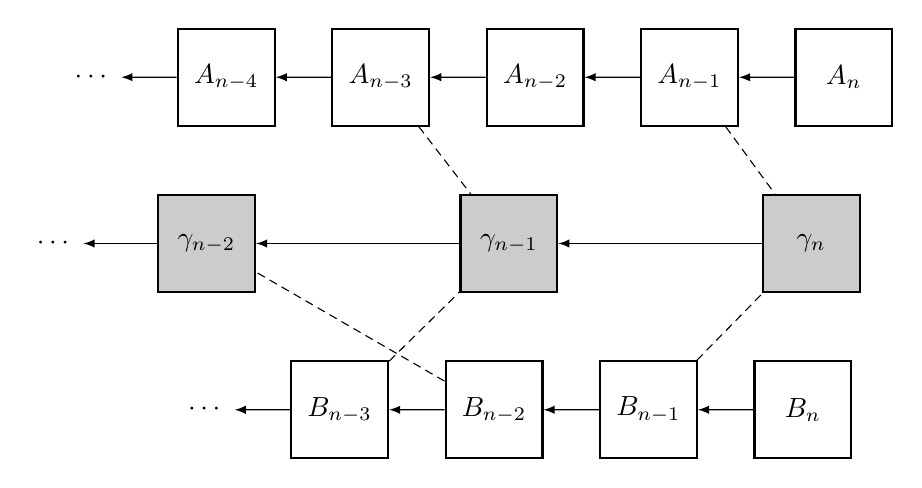
\begin{tikzpicture}[scale=0.96]
    \tikzstyle{root} = [draw=black, thick, fill=black!20, rectangle, minimum height=3.5em, minimum width=3.5em, node distance=3em];
    \tikzstyle{org-block} = [draw, thick, fill=white, rectangle, minimum height=3.5em, minimum width=3.5em, node distance=2em];
    \tikzstyle{link} = [-, thin, densely dashed];
    \tikzstyle{pointer} = [thin, -latex];

    \node (org-a-0) at (-2.5, 2.2)                {$\cdots$};
    \node[org-block] (org-a-1) [right=of org-a-0] {$A_{n-4}$}
        edge [pointer] (org-a-0.east);
    \node[org-block] (org-a-2)  [right=of org-a-1] {$A_{n-3}$}
        edge [pointer] (org-a-1.east);
    \node[org-block] (org-a-3)  [right=of org-a-2] {$A_{n-2}$}
        edge [pointer] (org-a-2.east);
    \node[org-block] (org-a-4)  [right=of org-a-3] {$A_{n-1}$}
        edge [pointer] (org-a-3.east);
    \node[org-block] (org-a-5)  [right=of org-a-4] {$A_{n}$}
        edge [pointer] (org-a-4.east);

    \node (root-0) at (-3, 0)        {$\cdots$};
    \node (root-1) at (-1, 0) [root] {$\gamma_{n-2}$}
        edge [pointer] (root-0.east);
    \node (root-2) at ( 3, 0) [root] {$\gamma_{n-1}$}
        edge [pointer] (root-1.east);
    \node (root-3) at ( 7, 0) [root] {$\gamma_{n}$}
        edge [pointer] (root-2.east);

    \node (org-b-0) at (-1, -2.2) {$\cdots$};
    \node[org-block] (org-b-1) [right=of org-b-0] {$B_{n-3}$}
        edge [pointer] (org-b-0.east);
    \node[org-block] (org-b-2) [right=of org-b-1] {$B_{n-2}$}
        edge [pointer] (org-b-1.east);
    \node[org-block] (org-b-3) [right=of org-b-2] {$B_{n-1}$}
        edge [pointer] (org-b-2.east);
    \node[org-block] (org-b-4) [right=of org-b-3] {$B_{n}$}
        edge [pointer] (org-b-3.east);

    \draw [link] (org-a-2) -- (root-2);
    \draw [link] (org-a-4) -- (root-3);
    \draw [link] (org-b-2) -- (root-1);
    \draw [link] (org-b-1) -- (root-2);
    \draw [link] (org-b-3) -- (root-3);
\end{tikzpicture}
\end{document}

    \caption{Block-lattice design. $B_a$, $B_b$ and $B_c$ are chains partially ordered in relation to one another.\label{block-lattice}}
\end{figure}

Block-lattices are a replicated data-structure composed of chains of blocks,
depicted in Figure~\ref{block-lattice}.  Both parallel and synchronized
operations are able to be expressed with this design:  a pair of transactions
on two chains are considered \emph{free}, if they may be processed in parallel,
or \emph{dependent}, if a causal or acausal dependency exists between them.

Each chain in our design functions as a logical unit of organization,
governance, and funding. In other words, each user, organization or community
is expected to operate under their own chain. These individual chains are
called \emph{accounts}. The block-lattice design has numerous advantages for
our use case, including parallel transaction processing, logical sharding and
the ability to trivially fork individual communities or organizations.

\subsection{Threat Model}

We assume a majority ($> 50\%$) of honest, or \emph{compliant} nodes which follow
the protocol. In other words, for $f$ non-compliant (faulty) nodes, we assume a
network of $2f+1$ nodes in total.

\subsection{Blocks, State and Transactions}

In \S~\ref{operations-and-state}, we saw that the protocol semantics could
be defined in terms of a global state $\State$ and a sequence of operations
$\op_1 \dotso \op_n$ applied to $\State$, forming a ledger $\Ledger$. When
describing the network architecture and protocol, a direct mapping between
these abstract objects and the components of the software architecture exist.

\subsubsection{State}

The state $\State$ is represented by a function $\State : K \to V$ which maps a
set of keys $K \in \mathbb{B}^{256}$ to a set of values $V \in \mathbb{B}^{*}$,
where $\mathbb{B}$ is the set of bytes, and $\mathbb{B}^n$ is the set of byte
strings of length $n$. The initial state $\State_0$ is called the
\emph{genesis} state. Since we are working with multiple chains, and each
chain represents an account's ledger, we define $\mathcal{A}_i$ to be the state
of account $i$ and $\mathcal{L}_i$ to be $i$'s ledger.

\subsubsection{Block}

An operation $\op$ is represented by a sequence of one or more transactions,
organized in a \emph{block}. A ledger $\Ledger$ of all valid recorded
operations is represented as a sequence of blocks, or \emph{blockchain}. A
block $B$ in \oscoin{} consists of a block header $B_H$ with a set of fields
(Table~\ref{block-header-fields}.) and a sequence of transactions $B_T = (t_0
\dotso t_n)$.

% TODO: Is it zero or more txns?

\begin{table}[hbtp]
    \caption{Block header fields \label{block-header-fields}}
    \begin{tabular}{l c p{7.5cm}}
        \toprule
        Field                  & Notation & Description \\
        \midrule
        \emph{Chain}           & $H_{id}$ & The name or identifier of the chain, \eg ``oscoin.'' \\
        \emph{Height}          & $H_n$    & The block height. \\
        \emph{ParentHash}      & $H_p$    & The \hash{} hash of the parent block header. \\
        \emph{TransactionRoot} & $H_{tr}$ & The root of the transaction hash tree. \\
        \emph{StateRoot}       & $H_{sr}$ & The \hash{} hash of the root of the state
                                            tree after all transactions in the block have
                                            been applied. \\
        \emph{Author}          & $H_a$    & The author of the block, and address to which
                                            all transaction fees collected in this block
                                            should be sent. \\
        \emph{Timestamp}       & $H_t$    & The local time of the author of this block at
                                            the time of authorship. \\
        \emph{ConsensusHash}   & $H_c$    & The \hash{} hash of the consensus parameters
                                            with which to validate the next block. \\
        \bottomrule
    \end{tabular}
\end{table}

% TODO: Sender account has a nonce.

\subsubsection{``Free'' Transactions}

Transactions which can be validated and applied to the state $\State$
individually are called \emph{free}. Free transactions can always be processed
in parallel because the resulting state after applying a free transaction does
not need to be observed by other chains. Formally, if $t$ is a free transaction
on chain $a$, the resulting state $\State'[a] \equiv \apply(\State[a], t)$
is not observable by any chain $c$ where $c \neq a$.

With the exception of \textsc{open}, all transactions carry an implicit account
context $a$, to which they are applied.

\begin{description}
    \item[Open] $\tx{open}{a_{pk}, a_{gen}, a_{addr}}_{\sigma}$.  Open a new
        account. This is the first transaction any organization or user must
        submit to initialize their account and chain.  $a_{pk}$ is the public
        key of the user registering the account, $a_{gen}$ is the genesis state
        of the account, and $a_{addr}$ is its public address.  Once processed,
        this transaction functions as the ``genesis block'' of an account.
    \item[Fork] $\tx{fork}{k_c, k_{c'}}_\sigma \; \text{where} \; k_c =
        \mathcal{C}_{\varnothing}$. Create a new context $k_{c'}$ by forking
        the empty context $\mathcal{C}_{\varnothing}$. This transaction can
        be used to create new code repositories.
    \item[Issue] $\tx{issue}{i_{id}, i_{c}}_\sigma$. Open an issue. The $i_{id}$
        parameter is used to reference the issue in subsequent transactions,
        while $i_c$ is the context in which to create the issue.
    \item[Amend] $\tx{amend}{i_{id}, i_{s}, i_{b}, i_P}_\sigma$.
        Update an issue's subject, body or patchset.
    \item[Voice] $\tx{voice}{i_{id}, v}_\sigma$.  Adds a voice $v$ to the issue
        $i$, where $v \in \{accept, reject\}$.
    \item[Bond] $\tx{bond}{b_{s}, b_{r}, b_{v}}_{\sigma}$. Bond $b_v$ tokens
        from the source address $b_{s}$ to the bonding address $b_r$. The
        signature $\sigma$ is used to unlock $b_s$.
    \item[Unbond] $\tx{unbond}{b_{s}, b_{r}, b_{v}}_{\sigma}$. Start unbonding
        $b_v$ tokens from the bonding address $b_{s}$ and credit $b_r$ when
        the unbonding period is over. The signature $\sigma$ unlocks the
        bonded tokens in $b_s$.
    \item[Set] $\tx{set}{s_k, s_v}$. Set an arbitrary key $s_k$ to the value
        $s_v$.
\end{description}

\subsubsection{``Dependent'' Transactions}

Transactions which appear in pairs accross two accounts are called
\emph{dependent} (Figure~\ref{tx-dependencies}.), due to only being valid when
applied in pairs. Typically, these transactions affect both accounts and
require temporary synchronization for both transactions to be observed and
processed by a node.

\begin{figure}[hbp]
    \documentclass[tikz]{standalone}

\usetikzlibrary{fit}
\usetikzlibrary{positioning}
\usetikzlibrary{backgrounds}
\usetikzlibrary{arrows.meta}

\begin{document}
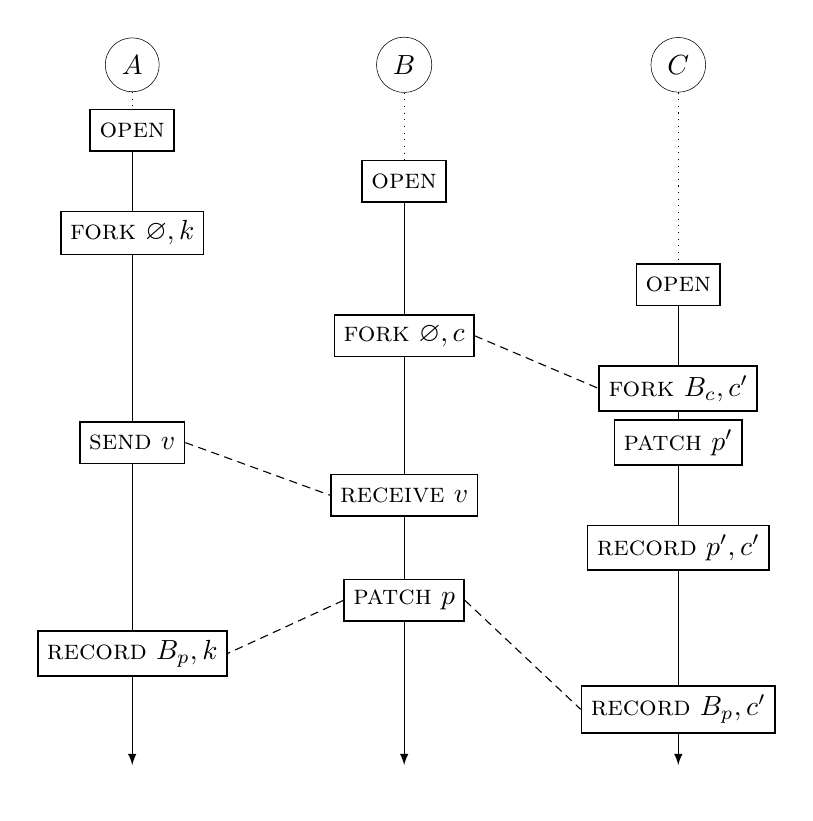
\begin{tikzpicture}
    \tikzstyle{link} = [-, thin, densely dashed];
    \tikzstyle{pointer} = [thin, -latex];
    \tikzstyle{account} = [draw, circle, font=\Small];
    \tikzstyle{tx} = [fill=white, rectangle, draw, semithick, minimum width=3em, minimum height=1.5em, font=\Small];
    \tikzstyle{end} = [];
    \tikzstyle{sync} = [-, densely dashed];

    \node [matrix, very thin, column sep=1.3cm, row sep=0.1cm] (matrix) at (0, 0) {
        \node[account] (A) {$A$};                         & \node[account] (B) {$B$};                         & \node[account] (C) {$C$};                    \\
                                                          &                                                   &                                              \\
        \node[tx] (A-open) {\textsc{open}};               &                                                   &                                              \\
                                                          & \node[tx] (B-open) {\textsc{open}};               &                                              \\
        \node[tx] (A-1) {\textsc{fork} $\varnothing, k$}; &                                                   &                                              \\
                                                          &                                                   & \node[tx] (C-open) {\textsc{open}};          \\
                                                          & \node[tx] (B-1) {\textsc{fork} $\varnothing, c$}; &                                              \\
                                                          &                                                   & \node[tx] (C-1) {\textsc{fork} $B_c, c'$};   \\
        \node[tx] (A-2) {\textsc{send} $v$};              &                                                   & \node[tx] (C-2) {\textsc{patch} $p'$};       \\
                                                          & \node[tx] (B-2) {\textsc{receive} $v$};           &                                              \\
                                                          &                                                   & \node[tx] (C-3) {\textsc{record} $p', c'$};  \\
                                                          & \node[tx] (B-3) {\textsc{patch} $p$};             &                                              \\
        \node[tx] (A-3) {\textsc{record} $B_p, k$};       &                                                   &                                              \\
                                                          &                                                   & \node[tx] (C-4) {\textsc{record} $B_p, c'$}; \\
                                                          &                                                   &                                              \\
                                                          &                                                   &                                              \\
                                                          &                                                   &                                              \\
        \node[end] (A-end) {};                            & \node[end] (B-end) {};                            & \node[end] (C-end) {};                       \\
    };

    \begin{scope}[on background layer]
        \draw[-, dotted] (B)        to (B-open);
        \draw[-, dotted] (C)        to (C-open);
        \draw[-, dotted] (A)        to (A-open);
        \draw[-latex]    (A-open)   to (A-end);
        \draw[-latex]    (B-open)   to (B-end);
        \draw[-latex]    (C-open)   to (C-end);
        \draw[sync]      (A-2.east) to (B-2.west);
        \draw[sync]      (B-1.east) to (C-1.west);
        \draw[sync]      (B-3.east) to (C-4.west);
        \draw[sync]      (B-3.west) to (A-3.east);
    \end{scope}
\end{tikzpicture}
\end{document}

    \caption{Three accounts, $A$, $B$ and $C$, and their transaction chains.
        The diagram illustrates free transactions, such as \textsc{open} and
        \textsc{patch}, as well as dependent transactions such as \textsc{send}
        and \textsc{receive}.  The dashed lines represent cross-chain
        synchronizations between dependent transactions.
    \label{tx-dependencies}}
\end{figure}

\begin{table}[hbtp]
    \begin{tabular}{l c p{7.5cm}}
        \toprule
        Field                  & Notation & Description \\
        \midrule
        \emph{Chain}           & $H_c$    & The name or identifier of the chain, \eg ``oscoin.'' \\
        \emph{Height}          & $H_n$    & The block height. \\
        \emph{ParentHash}      & $H_p$    & The \hash{} hash of the parent block header. \\
        \emph{TransactionRoot} & $H_{tr}$ & The root of the transaction hash tree. \\
        \emph{StateRoot}       & $H_{sr}$ & The \hash{} hash of the root of the state
                                            tree after all transactions in the block have
                                            been applied. \\
        \emph{Author}          & $H_a$    & The author of the block, and address to which
                                            all transaction fees collected in this block
                                            should be sent. \\
        \emph{Timestamp}       & $H_t$    & The local time of the author of this block at
                                            the time of authorship. \\
        \emph{ConsensusHash}   & $H_c$    & The \hash{} hash of the consensus parameters
                                            with which to validate the next block. \\
        \bottomrule
    \end{tabular}
    \medskip
    \caption{Block header fields \label{block-header-fields}}
\end{table}

\input{sections/light-clients.tex}
\input{sections/safety.tex}
\input{sections/incentivization.tex}
\input{sections/future-work.tex}

\section{Conclusion}

\end{multicols}

\appendix
\end{document}
